\multiplechoicestart


\spoergsmaal{Gode egenskaber ved algoritmer}
Hvilke af følgende egenskaber er typisk ønskelige for en algoritme?
\fleresvar
\mulighederstart
\svar Den kører hurtigt \korrekt
\svar Den bruger mest for-løkker og ingen eller meget få while-løkker
\svar Den udnytter al computerens hukommelse
\svar Den laver mange rekursive kald
\svar Den giver det ønskede resultat for alle mulige input \korrekt
\svar Den er svær at forstå, så ingen kan kopiere den
\mulighederslut
\forklaring{
Gode algoritmer er effektive (hurtige og med lavt hukommelsesforbrug) og giver det ønskede resultat i alle tilfælde. At bruge bestemte kontrolstrukturer, meget hukommelse eller gøre algoritmen unødigt kompleks er ikke ønskelige egenskaber.
}

\spoergsmaal{Sandsynligheder}
Hvilke af følgende tal kan være sandsynligheder?
\fleresvar
\mulighederstart
\svar $-2$
\svar $10^{-9}$ \korrekt
\svar $0.25$ \korrekt
\svar $1$ \korrekt
\svar $1.5$
\svar $2$
\svar $-0.5$
\mulighederslut
\forklaring{
En sandsynlighed er altid et tal i intervallet $[0,1]$. Negative tal og tal større end $1$ kan ikke være sandsynligheder.
}

\spoergsmaal{Antal rækkefølger}
Vi har 10 forskellige spillekort liggende i en hat. Vi trækker et kort og lægger det tilbage, og det gør vi 5 gange. Hvor mange forskellige rækkefølger af 5 kort er der mulighed for?
\etsvar
\mulighederstart
\svar $5^{10}$
\svar $\binom{10}{5}$
\itxsvar{binom(10,5)}
\svar $5!$
\svar $10!$
\svar $10^5$ \korrekt
\mulighederslut
\forklaring{
Ved hvert af de 5 træk har vi 10 mulige kort.
Antallet af mulige rækkefølger er derfor $10^5$.
}

\spoergsmaal{Egenskaber ved grafer}
Hvilke af følgende ord beskriver egenskaber ved grafer?
\fleresvar
\mulighederstart
\svar sammenhængende \korrekt
\svar harmonisk
\svar isotropisk
\svar orienteret \korrekt
\svar projektiv
\svar acyklisk \korrekt
\mulighederslut
\forklaring{
Typiske egenskaber ved grafer er sammenhængende (connected), orienteret (directed) og acyklisk (acyclic).
}


\spoergsmaal{Basale pseudokode-ord}
Hvilke af følgende ord bruger vi ofte i basal pseudokode?
\fleresvar
\mulighederstart
\svar so
\svar must
\svar prioritize
\svar else \korrekt
\svar while \korrekt
\mulighederslut
\forklaring{
I pseudokode bruges kontrolstrukturer som while og else.
De andre ord bruger vi ikke i pseudokode.
}


\spoergsmaal{Datastrukturer fra pensum}
Hvilke af følgende ord er navne på datastrukturer fra kursets pensum?
\fleresvar
\mulighederstart
\svar index-træ
\svar stak \korrekt
\svar hob \korrekt
\svar container
\svar hyperliste
\svar gruppe
\mulighederslut
\forklaring{
I kurset har vi lært om stakke og hobe.
De andre ord er ikke standard datastrukturer.
}

\spoergsmaal{Egenskaber ved max-hobe}
Hvilke af følgende udsagn passer for enhver max-hob?
\fleresvar
\mulighederstart
\svar Roden har den mindste værdi
\svar Højst én knude har netop ét barn \korrekt
\svar Højden af træet (antallet af kanter på den længste sti fra et blad til roden) er  ikke $\Omega(n)$ \korrekt
\svar Der er ikke flere knuder med samme værdi
\svar Alle blade har samme dybde (afstand til roden)
\svar Hvis der er $n$ knuder, så er der $\lceil n/2\rceil$ blade. \korrekt
\mulighederslut
\forklaring{
En max-hob er et komplet binært træ, hvor roden indeholder den største værdi, og hver forælder er større end eller lig med sine børn.
Højden er $\Theta(\log n)$, ikke $\Omega(n)$. Der kan være dubletter.
Højst én knude kan have ét barn (på sidste niveau), ellers er der et uudfyldt niveau.
Alle blade har ikke nødvendigvis samme dybde, der kan være en forskel på 1.
Der er $\lceil n/2\rceil$ blade.
}

\spoergsmaal{Operationer i en prioritetskø}
Hvilke af følgende operationer understøttes typisk af en max-prioritetskø?
\fleresvar
\mulighederstart
\svar \proc{Invert-Priority}
\svar \proc{Shuffle-All}
\svar \proc{Downgrade}
\svar \proc{Insert} \korrekt
\svar \proc{Extract-Max} \korrekt
\mulighederslut
\forklaring{
En prioritetskø understøtter typisk operationer som \texttt{Insert} og \texttt{Extract-Max}.
}

\spoergsmaal{Egenskaber ved relationer}
Hvilke af følgende ord er egenskaber ved en relation?
\fleresvar
\mulighederstart
\svar kommutativ
\svar antisymmetrisk \korrekt
\svar hyperrefleksiv
\svar symmetrisk \korrekt
\svar positiv
\svar kontradiktorisk
\mulighederslut
\forklaring{
Symmetrisk og antisymmetrisk er egenskaber ved relationer, ikke de andre ord.
}

\spoergsmaal{Sorteringsalgoritmer fra pensum}
Hvilke af følgende er sorteringsalgoritmer fra kursets pensum?
\fleresvar
\mulighederstart
\svar fast sort
\svar radix sort \korrekt
\svar power sort
\svar deletion sort
\svar heap sort \korrekt
\mulighederslut
\forklaring{
Heap sort og radix sort er klassiske sorteringsalgoritmer fra pensum.
}

\spoergsmaal{Transitiv relation}
Lad $X$ være en mængde og lad $R \subseteq X \times X$ være en relation på $X$.
Hvad betyder det at $R$ er transitiv?
\etsvar
\mulighederstart
\svar Hvis $(a,b) \in R$, så er $(b,a) \in R$
\svar Hvis $(a,b) \in R$, så er $(a,a) \in R$
\svar Hvis $(a,b) \in R$ og $(b,c) \in R$, så er $(c,a) \in R$
\svar Hvis $(a,b) \in R$, så er $(a,c) \in R$ for alle $c \in X$
\svar Hvis $(a,b) \in R$ og $(b,c) \in R$, så er $(a,c) \in R$ \korrekt
\mulighederslut
\forklaring{
En relation $R$ er transitiv, hvis for alle $a,b,c \in X$ gælder: $(a,b) \in R$ og $(b,c) \in R \implies (a,c) \in R$. De andre udsagn beskriver symmetri, refleksivitet eller unavngivne egenskaber.
}


\spoergsmaal{Pseudokode 1}
Betragt følgende pseudokode
\begin{codebox}
\Procname{$\proc{For-Loop}(x)$}
\li $S \gets 1$
\li \For $i \gets 1$ \To $x$ \Do
\li \quad $S \gets 2 \cdot S + i$
    \End
\li \Return S
\end{codebox}
Hvad returneres når koden kaldes med input $x=3$?
\etsvar
\mulighederstart
\svar 8
\svar 14
\svar 19 \korrekt
\svar 25 
\svar 30
\mulighederslut
\forklaring{Før forloopet har vi $S=1$. Herefter sker følgende i hver iteration:
\begin{itemize}
    \item Iteration \(i = 1\): $S=2 \cdot 1+1=3$
    \item Iteration \(i = 2\): $S=2 \cdot 3+2=8$
    \item Iteration \(i = 3\): $S=2 \cdot 8+3=19$
\end{itemize}
}


\spoergsmaal{Sum}
Udregn følgende udtryk 
\begin{align*}
1 + 2 + 3 + \ldots + 99 + 100
\end{align*}
\etsvar
\mulighederstart
\svar 4852
\svar 4975
\svar 5013
\svar 5050 \korrekt
\svar 5087
\mulighederslut
\forklaring{
  Det er en klassisk historie at Gauss som barn
  løste overstående problem,
  ved at se at summen svarer til \(101\)
  50 gange.
  Mere generelt har vi
  \begin{align*}
      \sum_{i=1}^{n} i &= 1 + 2 + 3 + \ldots + n = \frac{n(n+1)}{2},
  \end{align*}
  som vi har lært tidligere i kurset.
}


\spoergsmaal{Pseudokode 2}
Betragt følgende pseudokode
\begin{codebox}
\Procname{$\proc{While-Loop}(x)$}
\li $y \gets 2 \cdot x$
\li \While $y \geq 6$ \Do
\li \quad \(y \gets y -6\)
    \End
\li \Return \(y\)
\end{codebox}
Hvilken funktion udregner pseudokoden, når $x$ er et ikke-negativt heltal?
\etsvar
\mulighederstart
\svar \(2 \cdot x\)
\svar \(2 \cdot x - 6\)
\svar \((2 \cdot x) \text{ mod } 6\) \korrekt
\svar \(\lfloor 2 \cdot x/6\rfloor\)
\svar \(\log_6(2\cdot x)\)
\mulighederslut
\forklaring{
While-loopet trækker $6$ fra $y$ indtil $y<6$, derfor udregner det \(y \bmod 6\).
Til at starte med har vi  \(y = 2 \cdot x\), så i alt udregnes \((2 \cdot x) \bmod 6\).
}

\sideskift



\spoergsmaal{Asymptotisk Analyse}
Betragt funktionen
\begin{align*}
  f(x) = x\log(x)^{2} +3x^4 + 5x^3 + 2x^2
\end{align*}
Hvilke af følgende udsagn om \(f\) er korrekte?
\fleresvar

\mulighederstart
\svar \(f = O(x^{4})\) \korrekt
\svar \(f = O(x^{5})\) \korrekt
\svar \(f = \Omega(x^{5})\)
\svar \(f = \Omega(x^{4}/\log x)\) \korrekt
\svar \(f = \Theta(x^{4}/\log x)\) 
\svar \(f = \Theta(x^{5})\)        
\mulighederslut
\forklaring{
  Den dominerende term i \(f\) er \(3x^{4}\).
  Derfor er \(f = O(x^{4})\) og \(f = O(x^{5})\).
  Da \(f\) vokser langsommere end \(x^{5}\) er \(f \neq \Omega(x^{5})\).
  Da \(f\) vokser hurtigere end \(x^{4}/\log x\) er \(f = \Omega(x^{4}/\log x)\).
}


\spoergsmaal{Repræsentation af hægtet liste i array}
Hvilken hægtet liste \(L\) repræsenteres af dette array \(A\)? Pointeren \(L.\text{head}\) (dvs.~index på det første listeelement) står i \(A[0]\).
Hvert listeelement gemmes i to nabofelter \(A[i]\) og \(A[i+1]\), hvor \(A[i]\) indeholder
nøgleværdien og \(A[i+1]\) indeholder en pointer (index) til det næste listeelement.

\begin{align*}
  A[0:8] = \langle 7, 9, \text{NIL}, 7, 1, 2, 3, 4, 5 \rangle
\end{align*}

\etsvar
\mulighederstart
\svar \(4 \rightarrow 2 \rightarrow 7 \rightarrow 9\) \korrekt
\svar \(4 \rightarrow 7 \rightarrow 2 \rightarrow 9\)
\svar \(7 \rightarrow 2 \rightarrow 4 \rightarrow 9\)
\svar \(7 \rightarrow 9 \rightarrow 2 \rightarrow 4\)
\svar Dette array definerer ikke nogen liste.
\mulighederslut
\forklaring{
  Pointeren \(L.\text{head}\) står i \(A[0]\), så vi starter ved index \(7\).
  \begin{itemize}
    \item Ved index \(7\) står nøglen \(A[7] = 4\) og pointeren \(A[8] = 5\).
    \item Ved index \(5\) står nøglen \(A[5] = 2\) og pointeren \(A[6] = 3\).
    \item Ved index \(3\) står nøglen \(A[3] = 7\) og pointeren \(A[4] = 1\).
    \item Ved index \(1\) står nøglen \(A[1] = 9\) og pointeren \(A[2] = \text{NIL}\), så listen slutter her.
  \end{itemize}
  Derfor repræsenterer arrayet listen
  \begin{align*}
          4 \rightarrow 2 \rightarrow 7 \rightarrow 9.
  \end{align*}
}

\sideskift

\spoergsmaal{Negation af udsagn}
Hvad er negationen af følgende udsagn?
\begin{align*}
  \exists x \in X \; \forall y \in Y : x \cdot y \le 1.
\end{align*}
\etsvar

\mulighederstart
\svar \(\exists x \in X \; \forall y \in Y : x \cdot y > 1\)
\itxsvar{\exists x \in X  \forall y \in Y : x * y > 1}
\svar \(\exists x \in X \; \forall y \in Y : x \cdot y \geq 1\)
\itxsvar{\exists x \in X \forall y \in Y : x * y >= 1}
\svar \(\exists x \in X \; \exists y \in Y : x \cdot y > 1\)
\itxsvar{\exists x \in X \exists y \in Y : x * y > 1}
\svar \(\exists x \in X \; \exists y \in Y : x \cdot y \geq 1\)
\itxsvar{\exists x \in X \exists y \in Y : x * y >= 1}
\svar \(\forall x \in X \; \forall y \in Y : x \cdot y > 1\)
\itxsvar{\forall x \in X \forall y \in Y : x * y > 1}
\svar \(\forall x \in X \; \forall y \in Y : x \cdot y \geq 1\)
\itxsvar{\forall x \in X \forall y \in Y : x * y >= 1}
\svar \(\forall x \in X \; \exists y \in Y : x \cdot y > 1\) \korrekt
\itxsvar{\forall x \in X \exists y \in Y : x * y > 1}
\svar \(\forall x \in X \; \exists y \in Y : x \cdot y \geq 1\)
\itxsvar{\forall x \in X \exists y \in Y : x * y >= 1}
\mulighederslut
\forklaring{
  For at negere udsagnet, laves alle \(\exists\)
  om til \(\forall\) og omvendt, og den indre funktion \(x \cdot y \leq 1\)
  negeres, som bliver til \(x \cdot y > 1\).
}

\spoergsmaal{Logik}
Hvad er kontrapositionen af udsagnet
"Hvis en person er en ægte skotte, går de i kilt"?
\etsvar
\mulighederstart
\svar Hvis en person ikke går i kilt, så er de ikke en ægte skotte. \korrekt
\svar Hvis en person ikke er en ægte skotte, så går de ikke i kilt. 
\svar Der findes ingen ægte skotte som går i kilt.
\svar Der findes en ægte skotte der ikke går i kilt.
\svar Der findes en person der går i kilt, som ikke er en ægte skotte.
\mulighederslut
\forklaring{
Kontrapositionen af et udsagn på formen "Hvis P, så Q" er "Hvis ikke Q, så ikke P",
som er ækvivalent med det oprindelige udsagn.
}

\spoergsmaal{Max-Heap}
Du kører BUILD-MAX-HEAP på arrayet \(A[0: 6] = \langle 2, 9, 3, 1, 4, 8, 7 \rangle\).
Hvilken hob får du som resultat?
\etsvar
\mulighederstart
\svar \(\langle 9, 4, 8, 1, 2, 3, 7 \rangle\) \korrekt
\svar \(\langle 9, 8, 7, 4, 3, 2, 1 \rangle\)
\svar \(\langle 9, 7, 8, 1, 2, 3, 4 \rangle\)
\svar \(\langle 9, 8, 4, 3, 7, 1, 2 \rangle\)
\svar \(\langle 9, 8, 4, 3, 7, 2, 1 \rangle\)
\mulighederslut
\forklaring{
Start: $A = \langle 2, 9, 3, 1, 4, 8, 7 \rangle$

Efter $\proc{Max-Heapify}(A,2)$:
$\langle 2, 9, 8, 1, 4, 3, 7 \rangle$

Efter $\proc{Max-Heapify}(A,1)$:
$\langle 2, 9, 8, 1, 4, 3, 7 \rangle$

Efter $\proc{Max-Heapify}(A,0)$:
$\langle 9, 4, 8, 1, 2, 3, 7 \rangle$
}


\spoergsmaal{Pokerhænder}
Vi spiller med et almindeligt sæt på 52 spillekort uden jokere (4 kulører og værdier fra 1 til 13).
Der trækkes 5 kort uden tilbagelægning: først 2 kort og derefter 3 kort.
Et udfald består af de 2 første kort og de 3 sidste kort; rækkefølgen inden for hver af de to grupper er ligegyldig.
Hvor mange udfald findes der af denne type:
\begin{itemize}
\item De 2 første kort har værdier med en forskel på 1 (fx 7 og 8).
\item De 3 sidste kort har andre værdier end de 2 første kort, og de er alle hjerter.
\end{itemize}

\textbf{Eksempel på et sådant udfald:} Klør 7, Ruder 8 og derefter Hjerter 3, Hjerter 5, Hjerter 9.

\etsvar
\mulighederstart
\svar \(13 \cdot \binom{4}{2} \cdot \binom{11}{3}\)
\itxsvar{13 * binom(4,2) * binom(11,3)}
\svar \(12 \cdot \binom{4}{2} \cdot \binom{13}{3}\)
\itxsvar{12 * binom(4,2) * binom(13,3)}
\svar \(12 \cdot 4 \cdot 4 \cdot \binom{11}{3}\)\korrekt
\itxsvar{12 * 4 * 4 * binom(11,3)}
\svar \(13 \cdot 4 \cdot 4 \cdot \binom{13}{3}\)
\itxsvar{13 * 4 * 4 * binom(13,3)}
\mulighederslut

\forklaring{
Der er 12 mulige par af værdier med forskel 1 (fra $\{1,2\}$ til $\{12,13\}$).
For hvert par vælger vi en kulør til kortet med den laveste værdi og en kulør til kortet med den højeste værdi: \(4 \cdot 4\).
De 3 sidste kort skal være hjerter og have andre værdier end de to valgte, så vi vælger 3 ud af de 11 resterende værdier: \(\binom{11}{3}\).
Dermed får vi \(12 \cdot 4 \cdot 4 \cdot \binom{11}{3}\).
Da vi skelner mellem de 2 første og de 3 sidste kort, tælles hvert udfald præcis én gang.
(Tæller man i stedet hænder på 5 kort uden rækkefølge, kan samme hånd opfylde betingelserne på flere måder, fx Hjerter 7, Klør 8, Hjerter 9, Hjerter 2, Hjerter 4.)
}


%TODO:Add this one if there still needs more
\spoergsmaal{Skuffeprincip og Hashing}
Antag at vi har gemt \(n\) nøgler i en hash-tabel af længde \(m\).
I hver placering af tabellen er der en hægtet liste hvor vi gemmer alle de nøgler der sendes til den placering.
Hvilket af følgende udsagn kan vi udlede fra
skuffeprincippet?
\etsvar
\mulighederstart
\svar Der er en placering som mindst \(\lceil n/m \rceil\) nøgler bliver sendt til. \korrekt
\svar Der bliver sendt mindst \(\lfloor n/m \rfloor\) nøgler til hver placering.
\svar Der bliver sendt højst \(\lfloor n/m \rfloor\) nøgler til hver placering.
\svar Der bliver sendt højst \(\lceil n/m \rceil\) nøgler til hver placering.
\mulighederslut
\forklaring{
Placeringer i hash-tabellen svarer til skuffer,
og nøgler svarer til objekter der skal fordeles i skufferne.
}


\spoergsmaal{Markovs Ulighed}
Lad \(X\in[0,10]\) være en stokastisk variabel med $\mathbb E[X]=5$.
Hvilken øvre grænse kan vi få ved brug af Markovs ulighed for sandsynligheden
\begin{align*}
  \Pr(X \leq 2 )?
\end{align*}
\etsvar
\mulighederstart
\svar \(\frac{3}{8}\)
\svar \(\frac{2}{5}\)
\svar \(\frac{5}{8}\) \korrekt
\svar \(\frac{3}{5}\)
\mulighederslut
\forklaring{Observer at $\Pr(X\leq 2)=\Pr(10-X\geq 8)$.
Vi definerer derfor en ny stokastisk variable $Y=10-X\in[0,10]$, og bemærker at $\mathbb E[Y]=\mathbb E[10-X]=10-\mathbb E[X]=10-5=5$.
Markovs ulighed siger $\Pr(Y\geq c\cdot \mathbb E[Y])\leq 1/c$.
Vi vælger derfor $c=8/5$ og får $\Pr(Y\geq \frac 85\cdot \mathbb E[Y])=\Pr(Y\geq 8)\leq 5/8$.
}


\spoergsmaal{Cuckoo hashing}
I nedenstående hashtabel er der indsat 5 nøgler med cuckoo hashing som beskrevet i
forelæsningen. Pilene viser den alternative placering af hver nøgle, fx kan
\(A\) flyttes mellem position \(0\) og \(3\), \(B\) mellem \(1\) og \(4\), og
\(C\) mellem \(2\) og \(5\).

\begin{center}
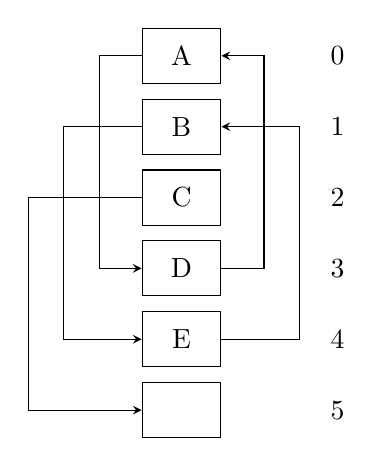
\begin{tikzpicture}[>=stealth,scale=0.9]
  \tikzstyle{slot}=[rectangle,draw,minimum width=1cm,minimum height=0.7cm,inner sep=0pt]

  % Slots (0..5)
  \node[slot] (s0) at (0,0) {A};
  \node[slot] (s1) at (0,-1) {B};
  \node[slot] (s2) at (0,-2) {C};
  \node[slot] (s3) at (0,-3) {D};
  \node[slot] (s4) at (0,-4) {E};
  \node[slot] (s5) at (0,-5) {};

  % Indices
  \node at (2.2,0) {0};
  \node at (2.2,-1) {1};
  \node at (2.2,-2) {2};
  \node at (2.2,-3) {3};
  \node at (2.2,-4) {4};
  \node at (2.2,-5) {5};

  % A <-> D (0 <-> 3)
  \draw[->] (s0.west) -- ++(-0.6,0) |- (s3.west);
  \draw[->] (s3.east) -- ++(0.6,0) |- (s0.east);

  % B <-> E (1 <-> 4)
  \draw[->] (s1.west) -- ++(-1.1,0) |- (s4.west);
  \draw[->] (s4.east) -- ++(1.1,0) |- (s1.east);

  % C <-> (tom) 5  (2 <-> 5)
  \draw[->] (s2.west) -- ++(-1.6,0) |- (s5.west);
\end{tikzpicture}
\end{center}

Vi indsætter nu en ny nøgle \(K\), hvor de mulige positioner er
\(h_{1}(K)=3\) og \(h_{2}(K)=2\), ved hjælp af standard cuckoo hashing,
hvilken hashtabel ender vi med?

\etsvar
\mulighederstart
\svar \(\langle D, B, K, A, E, C \rangle\) \korrekt
\svar \(\langle A, B, K, D, E, C \rangle\)
\svar \(\langle D, B, C, K, E, A \rangle\)
\svar \(\langle A, E, K, D, B, C \rangle\)
\svar Det er udefineret, da der vil opstå en uendelig løkke under indsættelsen, så der vil ske en rehashing.
\mulighederslut
\forklaring{
Indsættelsen forløber således:
\begin{itemize}
  \item \(K\) indsættes i position \(3\),
    så \(D\) fortrænges til sin alternative position \(0\).
  \item \(D\) indsættes i position \(0\),
    så \(A\) fortrænges til sin alternative position \(3\).
  \item \(A\) indsættes i position \(3\),
    så \(K\) fortrænges til sin alternative position \(2\).
  \item \(K\) indsættes i position \(2\),
    så \(C\) fortrænges til sin alternative position \(5\)
        som er tom. Da \(C\) bliver indsat på en tom plads, stopper indsættelsen her.
\end{itemize}
Den endelige tabel er derfor
\begin{align*}
  \langle D, B, K, A, E, C \rangle.
\end{align*}
}


\spoergsmaal{Matrixudregning}
Lad
\begin{align*}
    A =
\begin{bmatrix}
1 & 0\\
2 & 1\\
0 & 1
\end{bmatrix}
\quad \text{og} \quad
B =
\begin{bmatrix}
1 & 1\\
0 & 2\\
1 & 0
\end{bmatrix}.
\end{align*}

Beregn \(A^{T}B\). Her er \(A^{T}\) den transponerede af \(A\).

\etsvar
\mulighederstart
\svar \korrekt
\(\displaystyle
\begin{bmatrix}
1 & 5\\
1 & 2
\end{bmatrix}\)
\itxsvar{[[1,5],[1,2]]}

\svar \(\displaystyle
\begin{bmatrix}
1 & 1\\
5 & 2
\end{bmatrix}\)
\itxsvar{[[1,1],[5,2]]}

\svar \(\displaystyle
\begin{bmatrix}
1 & 5\\
0 & 3
\end{bmatrix}\)
\itxsvar{[[1,5],[0,3]]}

\svar \(\displaystyle
\begin{bmatrix}
1 & 0\\
5 & 3
\end{bmatrix}\)
\itxsvar{[[1,0],[5,3]]}

\mulighederslut
\forklaring{
Vi har
\begin{align*}
    A^{T} =
\begin{bmatrix}
1 & 2 & 0\\
0 & 1 & 1
\end{bmatrix}.
\end{align*}

Dermed er

\begin{align*}
    A^{T}B =
\begin{bmatrix}
1 & 2 & 0\\
0 & 1 & 1
\end{bmatrix}
\begin{bmatrix}
1 & 1\\
0 & 2\\
1 & 0
\end{bmatrix}
=
\begin{bmatrix}
1\cdot1 + 2\cdot0 + 0\cdot1 & 1\cdot1 + 2\cdot2 + 0\cdot0\\
0\cdot1 + 1\cdot0 + 1\cdot1 & 0\cdot1 + 1\cdot2 + 1\cdot0
\end{bmatrix}
=
\begin{bmatrix}
1 & 5\\
1 & 2
\end{bmatrix}.
\end{align*}

}


\spoergsmaal{Dijkstras algoritme}
Betragt den følgende vægtede, orienterede graf:

\begin{center}
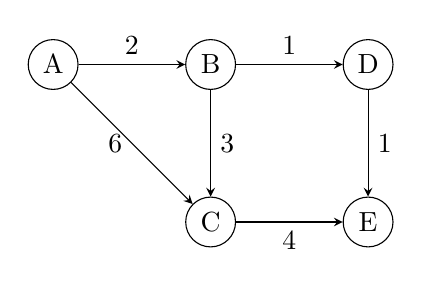
\begin{tikzpicture}[>=stealth, node distance=2.4cm]
  \tikzstyle{vertex}=[circle,draw,minimum size=18pt,inner sep=0pt]

  \node[vertex] (A) at (0,0) {A};
  \node[vertex] (B) at (2,0) {B};
  \node[vertex] (C) at (2,-2) {C};
  \node[vertex] (E) at (4,-2) {E};
  \node[vertex] (D) at (4,0) {D};

  \draw[->] (A) -- node[above] {2} (B);
  \draw[->] (A) -- node[left] {6} (C);
  \draw[->] (B) -- node[right] {3} (C);
  \draw[->] (B) -- node[above] {1} (D);
  \draw[->] (C) -- node[below] {4} (E);
  \draw[->] (D) -- node[right] {1} (E);
\end{tikzpicture}
\end{center}

Antag Dijkstras algoritme anvendes til at finde korteste veje fra knuden \(A\)
til alle knuder i grafen.
Angiv i hvilken rækkefølge knuderne bliver taget ud af
prioritetskøen i Dijkstras algoritme.
\etsvar

\mulighederstart
\svar \(A C B D E\)
\svar \(A C E B D\)
\svar \(A B C D E\)
\svar \(A B D E C\) \korrekt
\mulighederslut
\forklaring{
  \begin{itemize}
      \item Start: \(d(A)=0\), alle andre \(\infty\).  
      \item Fra \(A\): \(d(B)=2\), \(d(C)=6\). Næste knude er \(B\) (mindst afstand).  
\item Fra \(B\): \(d(C)\) forbedres til \(2+3=5\), \(d(D)=2+1=3\).  
\item Næste knude er \(D\) (afstand \(3\)), som giver \(d(E)=3+1=4\).  
\item Næste knude er \(E\) (afstand \(4\)).
\item Sidste knude er \(C\) (afstand \(5\)).
\end{itemize}
Rækkefølgen er derfor \(A,B,D,E,C\).
}






%TODO:Har ikke lavet noget om Uge 11. Man kunne enten lave noget om
%disjunkte mængder eller om amortiseret analyse.
\multiplechoiceslut

\label{page:last}
